%========================================================================================================================
%========================================================================================================================
%========================================================================================================================
\section{Semantics}
\label{sec:semantics}
In this section we formalize our consistency enforcement algorithm with an
operational semantics, which is also a high-level abstraction of our
tool \tool.
Our approach is complete for the specification language defined
in section \ref{sec:ctrt_language}, however, here for simplicity reasons we present an operational semantics 
parametrized over a contract with a single prop. As we will explain
in section \ref{subsec:generalization}, the rules can be easily
generalized to cover multiple consistency levels, each specified by any
given contract. Therefore, in the rest of this section we will assume a given contract $\psi$ of the
following form:
\begin{smathpar}
\begin{array}{llc}
\psi = \forall a. a \xrightarrow{R} \hat{\eta} \Rightarrow a 
\xrightarrow{\visZ} \hat{\eta}
& & R = r_1;r_2;...;r_k 
\quad
\end{array}
\end{smathpar}

The operational semantics is defined via a small-step relation over \emph{execution
states}, which are tuples of the form $\E=(\EffSoup,\visZ ,\soZ)$.
The \emph{effect soup} $\E.\EffSoup$, represents the set of all
effects produced in the system, and  $\E.\visZ$,
$\E.\soZ$ $\subseteq \EffSoup \times \EffSoup$, stand for, respectively the
visibility and session order relations
Among such effects. Figures \ref{subfig:execution_graph} and
\ref{subfig:execution_example} represent a simple
execution state of the system consisting of 9 effects with associated
primitive relations, where we ommited drawing the transitive $\soZ$ edge between
$\eff_8$ and $\eff_1$, for better readability.
\begin{figure}[h]
	
	\begin{subfigure}[b]{0.28 \textwidth}
	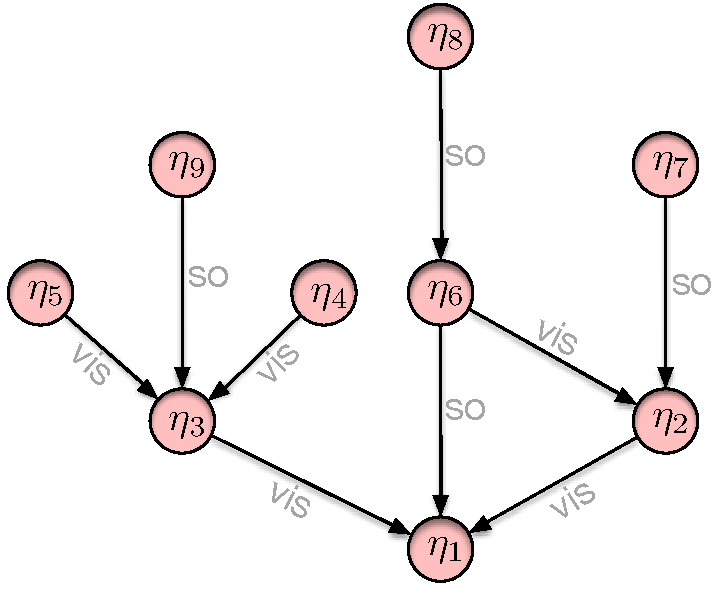
\includegraphics[scale=0.38]{Figures/execution.pdf}
	\subcaption{An execution state \E}
	\label{subfig:execution_graph}
	\end{subfigure}
	%
	\quad \vrule \quad
	%
	\begin{subfigure}[b]{0.31 \textwidth}
	\begin{smathpar}
	\begin{array}{lcl}
	\E.\EffSoup & = & 
	\{\eta_1,\eta_2,\eta_3,\eta_4,\eta_5,\eta_6,\eta_7,\\ & & \;\eta_8,\eta_9\}\\
	\E.\visZ & = & 
	\{(\eta_5,\eta_3),(\eta_4,\eta_3),(\eta_3,\eta_1),\\ &
	&\;(\eta_2,\eta_1),(\eta_6,\eta_2)\} \\ 
	\E.\soZ & = & \{(\eta_9,\eta_3),(\eta_8,\eta_6),(\eta_6,\eta_1),\\ 
	& & \;(\eta_8,\eta_1),(\eta_7,\eta_2) \} \\ 
	\end{array}
	\end{smathpar}\\
	\subcaption{Effect soup and primitive relations}
	\label{subfig:execution_example}
	\end{subfigure}
	%
	\quad \vrule \quad
	%
	\begin{subfigure}[b]{0.3 \textwidth}
	\begin{smathpar}
	\begin{array}{lll}
	\visZ^{-1}  (\eta_1) & = & \{\eta_2,\eta_3\} \\ 
	\soZ^{-1}  (\eta_1) & = & \{\eta_6, \eta_8\} \\
	(\soZ\cup\visZ)^{-1} (\eta_1) & = &
	\{\eta_2,\eta_3,\eta_6,\eta_8\} \\ 
	(\visZ^*)^{-1} (\eta_1) & = &
	\{\eta_2,\eta_3,\eta_4,\eta_5,\eta_6\} \\ 
	(\soZ;\visZ)^{-1}(\eta_1) & = & \{\eta_7,\eta_9\}
	\\ \\
	\end{array}
	\end{smathpar} \\
	\subcaption{Relation inverse examples}
	\label{subfig:inverse_example}
	\end{subfigure}
	\caption{A simple execution state }
\label{fig:execution_state}
\end{figure}

We use notation $\EffSoup_{(condition)}$
to represent a  subset of $\EffSoup$ consisting of effects that
satisfy the specified condition.
Note that \tool's contracs are in fact constraints over execution states,
where the domain of quantification is fixed to the effect soup
$\EffSoup$, and
interpretation for $\soZ$ and $\visZ$ relations (which occur free in the
contract formulae) are also provided. Thus, execution states are
potential
models for any first-order formula expressable in the contract
language. If an execution state $\E$ is in fact a valid model for a contract
$\psi$, we say that $\E$ satisfies $\psi$, written as $\E
\models \psi$. 


The samentics' reduction step is of the form
\begin{smathpar}
(\E,\op_{<s,i>}) \;\xrightarrow{\V}\; (\E', \eff),
\end{smathpar}
which can be interpreted as a reduction with the initial execution state $\E$, caused by a replica with a local 
set of effects $\V$, after it executes an operation
$\op$, which is the $i$'th request from the session $s$. 
During this reduction step a new effect $\eff$ is produced and added to
the system, resulting a new execution state $\E'$ with updated effect
soup and primitive relations.

Before introducing the operational semantics, we will first formally
present the required definitions in the next section. Namely, we will define  
notions of the \emph{inverse} of a given relation $R$, and the \emph{maximally
closed subset} of a given set of effects $V$ under a contract $\psi$. 




%=============================================================================================================
%--------- Definitions to be used in the semanrics
%=============================================================================================================
\subsection{Preliminaries}
\label{subsec:prelim}
Firstly, we need to define the trancated relation for a given $R \in$
\relationS{} as a relation derived by removing the last element from the
sequence in $R$ (if there is any). i.e.
\begin{smathpar}
\trunc{R} = 
\begin{cases}
\begin{array}{lcl}
\nullR & \myif & R = \rel \quad \vee \quad R = \nullR \\
\rel^* & \myif & R = \rel^* \\ 
R' & \myif & R = R';\rel \\
R';\rel^* & \myif & R = R';\rel^*
\end{array}
\end{cases}
\end{smathpar}
We now continue by formally defining the inverse of a relation ($\rel \in$
\seedS{}) given an 
execution state $\E$:
\begin{smathpar}
\rel^{-1}(\Set) = 
\begin{cases}
\begin{array}{lcl}
\bigcup\limits_{\eta\in \Set}. \{\eta'|(\eta',\eta) \in \E.\rel \} & \myif
&\rel\in\{\soZ,\visZ\}\ \\ 
\rel_1^{-1}(\Set)\cup \rel_2^{-1}(\Set) & \myif & \rel=\rel_1\cup \rel_2
\end{array}
\end{cases}
\end{smathpar}
Note that when the input set of an inversed relation is a singleton
$\{\eta\}$, we drop the brackets and simply write it as
$\rel^{-1}(\eta)$.
Now, using a recursive function $G^\rel$, we extend the above definition to
the closure of $\rel$ as follows:
\begin{smathpar}
(\rel^{*})^{-1}(\Set) = G^{\rel}(\Set,\emptyset) 
\end{smathpar}
where,
\begin{smathpar}
G^\rel(\Set,P) =
\begin{cases}
\begin{array} {ll}
G^\rel(\rel^{-1}(\Set) , P\cup \rel^{-1}(\Set)) &\myif \; \rel^{-1}(\Set) \neq \emptyset  \\
P  &   \mathtt{otherwise} 
\end{array}
\end{cases}
\end{smathpar}
For example, in figure \ref{subfig:inverse_example} (where the inverse
of various different relations are presented),
$(\visZ^*)^{-1}(\eta_1)$ is computed by first calling
$G^{\visZ}(\{\eta_1\},\emptyset)$ which returns
$G^{\visZ}(\{\eta_2,\eta_3\},\{\eta_2,\eta_3\}) $,
since $\visZ^{-1}(\eta_1) = \{\eta_2,\eta_3\} \neq \emptyset$.
Similarly, the second recursive call will result in
$G^{\visZ}(\{\eta_4,\eta_5,\eta_6\},\{\eta_2,\eta_3,\eta_4,\eta_5,\eta_6\})
$ where the computation reaches its fixed point, since  $\visZ^{-1}(\{\eta_4,\eta_5,\eta_6\}) =
\emptyset$, and final result of $\{\eta_2,\eta_3,\eta_4,\eta_5,\eta_6\}$ is returned.

We now present the definition of the inverse of 
a sequence (of size larger than 1) of \seedS{} and their clousres as follows:
\begin{smathpar}
\begin{array}{lllllrr}
\eta' \in  (R';r)^{-1}(\eta) & \iff & \exists \eta''. \eta'' \in r^{-1}(\eta)
& \wedge & \eta' \in (R')^{-1}(\eta'') & \qquad & (1)
\end{array}
\end{smathpar}
Note that, since $R\in$ \relationS{} in our specification language is
 either a \seedS{}, its clousre or a sequence of them, we are
now ready to formally define the inverse of any given relation $R$.
However, the above definitions do not capture the reality of distributed
systems, where the inverse of the relations are used by replicas, which
might have access to only a \emph{subset of all effects} at any given
moment. For example, consider  $(\soZ;\visZ)^{-1}(\eta_1)$ of the
execution state in figure
\ref{fig:execution_state}. In order to compute this set, based on the
recursive defintion of (1) we have: 
\begin{smathpar}
\begin{array}{lllll}
\eta' \in  (\soZ;\visZ)^{-1}(\eta_1) & \iff & \exists \eta''. \eta'' \in
\visZ^{-1}(\eta_1)
& \wedge & \eta' \in (\soZ)^{-1}(\eta'')
\end{array}
\end{smathpar}
Since
there exist \emph{mid-level} effects $\eta_2$ and $\eta_3$, such that satisfy the above
definition respectively 
for $\eta_7$ and $\eta_9$, we have: $(\soZ;\visZ)^{-1}(\eta_1) =
\{\eta_7,\eta_9\}$.
Now assume a replica only contains $\{\eta_1, \eta_6, \eta_7, \eta_8,
\eta_9\}$ and wants to check if the dependencies of $\eta_1$ are present
at the replica or not. Even though based on the above definitions the
answer is yes (since the replica contains $\{\eta_7,\eta_9\}$), but in
reality the replica is unable to verify that, since the mid-level
effects $\eta_2$ and $\eta_3$ are not present at the replica yet. 

To avoid the above problem, we now partially define the inverse of a given relation $R \in$
\relationS{} \emph{according to a set of available effects $V$}, only if all the required mid-level effects are
also present in $V$. We present a new version of the 
definition (1), based on a slightly modified helping function $G^\rel_V$.
\begin{smathpar}
\eta' \in (R)^{-1}_V(\eta) \iff
\begin{cases}
\begin{array} {lllll} 
\bot & \myif & R = \nullR& & \\
\eta' \in \rel^{-1}(\eta) & \myif & R=\rel & & \\
\eta' \in G^{\rel}_V(\{\eta\},\emptyset)  & \myif & R=\rel^* & & \quad
\qquad (2)  \\
\exists \eta''. \eta'' \in
\rel^{-1}(\eta) \wedge \eta' \in (R')^{-1}(\eta'') \wedge
\rel^{-1}(\eta) \subseteq V   & \myif & R=R';\rel & & 
\end{array}
\end{cases}
\end{smathpar}
Note that the last conjunct is the only difference between the third
line above and definition (1) which assures the presence of mid-level
effects before performing the next recursive call.  
%COMMENTCOMMENTCOMMENTCOMMENT
%
\begin{comment}
Simliarly, We define
$G_V^{\rel}$ as follows:
\begin{smathpar}
G_V^\rel(\Set,P) =
\begin{cases}
\begin{array} {lll}
G^\rel(\rel^{-1}(\Set) , P\cup \rel^{-1}(\Set)) &\myif & \rel^{-1}(\Set)
\neq \emptyset  \wedge \rel^{-1}(\Set) \subseteq V \\
\emptyset & \myif & \rel^{-1}(\Set) \neq \emptyset \wedge
\rel^{-1}(\Set) \not\subseteq V     \\
P  &   \myif & \rel^{-1}(\Set) = \emptyset 
\empty
\end{array}
\end{cases}
\end{smathpar}
\end{comment}
%COMMENTCOMMENTCOMMENTCOMMENT

Fainally, we define closed subsets of a given set of
effects $V$ under the contract $\psi$, which will be used to define the
the maximal of such subsets  (We will abuse the notation slightly
and use a \emph{set} as the input to the inverse relation, which simply is
the union of the inverse of the relation on all the elements in the
set):
\begin{smathpar}
\begin{array}{rlllll}
\mathtt{closed \; subsets:} &  V' \in \left \lfloor  V \right \rfloor & \iff & V' \subseteq V & \wedge &
(\trunc R)_V^{-1}(V') \subseteq V'   \\
\mathtt{maximally \; closed \; subset:} & V' = \left \lfloor  V \right
\rfloor_{\mathtt{max}} & \iff & V' \in \left \lfloor  V \right \rfloor &
\wedge & \not\exists V'' \in \left \lfloor  V \right \rfloor. |V''|>|V'|
\end{array}
\end{smathpar}


%=============================================================================================================
%--------- The operational semantics
%=============================================================================================================
\subsection{Core Operational Semantics}
\begin{figure}[t]
\raggedright
\textbf{Auxiliary Definitions}\\ \vspace{-2mm}
%
\begin{minipage}{0.5\textwidth}
\begin{fmathpar}
\begin{array}{lclcl}
  \multicolumn{5}{c}{
    {op} \in \mathtt{Operation\; Name} \spc \spc
    {v} \in \mathtt{Return\; Value} \spc \spc
    {s} \in \mathtt{Session\; Id} \spc\spc
  } 
  \\ 
  \eff & \in & \mathtt{Effect} & \coloneqq &  (s,op,v)\\
  F_{op} & \in & \mathtt{Op.\,Def.} & \coloneqq & \set{\eff} \mapsto v\\
  \EffSoup & \in & \mathtt{Eff\,Soup}	  & \coloneqq & \set{\eff} \\
  \visZ,\soZ &	\in & \mathtt{Relations} & \coloneqq & \set{(\eff,\eff)} \\
  {\E} 	& \in & \mathtt{Exec\;State}  & \coloneqq & \Exec \\
\end{array}
\end{fmathpar}
\end{minipage}
%

\vspace {3mm}

\textbf{Auxiliary Reduction} \; \\
\fcolorbox{black}{pgrey}{\scriptsize \(\auxred{S} {(\E,op_{<s,i>})} {} {(\E',\eff)}\)}\\
\begin{minipage}{0.9\textwidth}
\vspace{2mm}
\rulelabel{Oper}
\vspace{-2mm}
\begin{fmathpar}
\stretcharraybig
\begin{array}{l}
\RuleTwo
{
%\Theta(\rho \mapsto (v,cache)) \qquad
S \subseteq \EffSoup \qquad F_{op}(S) = v \qquad
\eta \not\in S \qquad
\eff = (s,op,v) \qquad  \\
%\id(\eta) = i \qquad
%\{\eff'\} = \EffSoup_{({\sf SessID}=s,\,{\sf SeqNo}=i-1)}\\
\EffSoup' = \EffSoup \cup \{\eff\}  \qquad
\visZ' = \visZ \cup S \times\{\eff\}\qquad
\soZ' = \soZ \cup \{(\eta',\eta) \,|\, \eta'\in \EffSoup_{({\sf
SessID}=s)}      \}\qquad
%\soZ' = (\soZ^{-1}(\eff') \cup \eff') \times\{\eff\} \cup \soZ
}
{
  \auxred {S} {((\EffSoup,\visZ,\soZ), op_{<s,i>}))}
  {} {((\EffSoup',\visZ',\soZ'),\eta)}
}
\end{array}
\end{fmathpar}
\end{minipage}
\vspace{4mm}\\
\textbf{Operational Semantics} \; \\
  \fcolorbox{black}{pgrey}{\scriptsize \((\E,op_{<s,i>}) \;\xrightarrow{V}\; (\E',\eff)\)}\\
\vspace{2mm}
\begin{minipage}{0.45\textwidth}
\rulelabel{UB Exec}
\vspace{-2mm}
\begin{fmathpar}
\stretcharraybig
\begin{array}{l}
\RuleTwo
{
  \visZ \subseteq r_k \spc
  V \subseteq E.A \spc  
  V'= \left \lfloor V \right \rfloor_V \spc
  \\ %   R^{-1}_{V}(\eta) \subseteq V' \\
  \auxred {V'} {(E, op_{<s,i>}))}
    {} {(E',\eta)} 
}
{
  (\E,op_{<s,i>}) \;\xrightarrow{V}\; (\E', \eff)
}
\end{array}
\end{fmathpar}
\end{minipage}
\hfill
\begin{minipage}{0.45\textwidth}
\rulelabel{LB Exec}
\vspace{-2mm}
\begin{fmathpar}
\stretcharraybig
\begin{array}{l}
\RuleTwo
{
     \visZ \not\subseteq r_k \spc
     V \subseteq E.A \spc  
     R^{-1}_{V}(\eta) \subseteq V \\
  \auxred {V} {(E, op_{<s,i>}))}
    {} {(E',\eta)} 
}
{
  (\E,op_{<s,i>}) \;\xrightarrow{V}\; (\E', \eff)
}
\end{array}
\end{fmathpar}
\end{minipage}
\\
\vspace{5mm}
\hrulefill\\
\caption{Core Operational semantics of a replicated data store.}
\label{fig:semantics}
\end{figure}

 %--- The Figure Containing the Rules

%--- Section intro
In this part we present the reduction rules, representing our
consistency preservation approach.
Figure \ref{fig:semantics} presents the set of rules defining the
auxiliary relation ($\hookrightarrow$) and small-step reduction relation 
($\rightarrow$) over executions. The latter relation is parametrized
over a set $V$,
that represents the set of effects that are available at the replica
that is 
taking the step. Obviously $V$ must be a subset of the effect soup 
of the initial execution, however, there is no other restrictions on $V$,
since we only assume eventual consistency at the underlying store.

%--- The [OPER] rule
Let's now go over the auxiliary reduction rule
\rulelabel{oper},
that represtns the procedure of producing a new effect $\eff$, by witnessing a set
of effects $S$. 
An effect is formally defined as a tuple $\eff=(s,op,v)$, representing the
session and the operation name 
whose execution creates $\eff$, and the state value
that the replica returns as the response to that operation.
The rule explains how the execution state changes after producing an
effect at a replica. Specifially, in the new state, the effect soup
$\EffSoup'$ must
now contain the newly created effect $\eff$, and the relations $\visZ'$
and $\soZ'$ must capture the fact that the set $S$ was made
visible to $\eta$, and all effects from the same session that were
already presenet in the intial execution state, should be in session
order with $\eff$ in the final execution state.


%--- rule for (->) relation
Now we explain the rule for reduction relation $(\xrightarrow{V})$,
namely \rulelabel{exec}, which represents the execution of operations
in a replica that updates the global state and produces a new
effect. The rule is crafted so it would only take place, if the
opertaing replica, contains the necessary effects specified by LB
contracts, and only allows the operations to witness effects that would
not violate the UB contracs.



%--- Explaining the operational rules
The preconditions of the reduction rules, include an auxiliary
reduction, explaining the changes that occur in the execution state $\E$
when an operation is performed. 
Moreover, the rule contains
$R_V^{-1}(\eff)\subseteq V'$ precondition, which basically guarantees
that the operation will witness the set of necessary effects, specified
by an LB contract. Note that this precondition trivially holds for UB
contracts, which only put constraints on the effects that are
\emph{about to} be made
visible to $\eff$, unlike LB contracts that end with an $\soZ$ relation and
refer to an \emph{already defined} set of dependencies. 

Moreover, the we have the precondition $V' = \left \lfloor V \right
\rfloor_V$, which basically filters out the effects from V, that would
violate a UB contract. Similarly this condition is trivially held for LB
contracts, since $V'$ is
already consistent because of the above pre-condition. In this case,
since $V'$ has
to be maximal, it should be set equal to $V$. The \rulelabel{exec}
similarly handles hybrid contracts, by both blocking oprtations and
filtering updates.

%=============================================================================================================
%--------- Theorem on correctness of enforcement
%=============================================================================================================
\subsection{Soundness}
\label{subsec:sound}
Here, we present a meta-theoretic property showing that the given contract would never be
violated, if the execution is in a consistent state and takes a reduction
step. We start by defining what we mean by a consistent state of the
execution: 
%
%Subsection on the correctness of contract 
%
In order to prove a meta-theoretic correctness property for our
semantics, we first define a $\psi$-consistent set of effects $S$ given
a execution state $\E$ as follows:

\begin{equation}
\scriptsize
S \mathtt{\;is\;} \psi \mathtt{-consistent} \iff \forall (\eff \in S).
\forall(a\in \E.\EffSoup). \trunc{R}(a,\eta)
\Rightarrow a \in S
\end{equation}
%Where the definition of $R$ is based on the definition of $R^{-1}$ from
%subsection 
%\ref{subsec:prelim}:
%\begin{equation}
%\scriptsize
%R(a,b) \iff a \in R_{E.A}^{-1}(b)  
%\end{equation}
\begin{theorem}
\label{theorem:one}
For all reduction steps 
$
\scriptsize
\; (\E,op_{<s,i>}) 
    \xrightarrow{V}
  (\E',\eff)  
$,
\begin{fmathpar}
\begin{array}{ll}
(i) & \mathtt{if\;} V \mathtt{\;is\;} \psi \mathtt{-consistent\;} \mathtt{under\;} \E,
\mathtt{\;then\;}  V \cup \{\eta\} \mathtt{\;is\;} \psi\mathtt{-consistent \; under\;} E'  \\
(ii) & E' \models \psi[\eta/\hat{\eta}]
\end{array}
\end{fmathpar}



\end{theorem}
\begin{proof}
Appendix \ref{app:proof1}
\end{proof}







%=============================================================================================================
%--------- Theorem on maxVis and minWait
%=============================================================================================================
\subsection{Optimality}
\label{subsec:opt}
Now we will present two theorems, regarding the optimality of our
approach. Firstly, we show that there
cannot be a larger subset of local effects in a replica to be made
visible to an operation, than what
our reduction rules specify. Next, we will prove the liveness property
of our semantics, which guarantees that all replicas will take a step,
given the proper set of local effects. Considering the eventual delivery of all
updates, which is guaranteed by the underlying store, this theorem
guarantees  that our system would never get permanently stuck. 
%
%Subsection of the maximality of the set made visible and liveness
%properties 
%
\begin{theorem}
\label{theorem:two}
For all reduction steps
{\footnotesize $
(\E,op_{<s,i>}) 
    \xrightarrow{V}
  (\E',\eff) 
$},
the set of effects made visible to $\eta$ is maximal. i.e. for all
 {\footnotesize $a \in V$}, if 
 {\footnotesize $ \SC {\trunc{R}} a V$}, then 
\begin{fmathpar}
(a,\eta) \not\in \E'.\visZ \Rightarrow 
(\E'.A,\E'.\visZ \cup \{a,\eta\}, \E'.so) \not\models \psi[\eta/\hat{\eta}]
\end{fmathpar}
\end{theorem}


%
% THE MINIIMAL WAIT THEOREM
%

\begin{theorem}
\label{theorem:three}
For all execution states $E$, if there
exists ($S\subseteq E.A$) such that: 
\begin{smathpar}
\auxred{S} {(\E,op_{<s,i>})} {} {(\E',\eff)} \spc \wedge \spc (\mathtt{S \cup \{\eta\} \; is 
\;} \psi \mathtt{-consistent \; under \;} E' )  
\end{smathpar}
then there exist  $E''$, $\eff'$ and $V\subseteq E.A$ such that:
$((\E,op_{<s,i>})\;\xrightarrow{V}\;(\E'',\eff'))$
\end{theorem}
\begin{proof}
The proof is given by choosing set $V$ to be equal to $S$, and then
considering two cases, where either $S$ or $\left \lfloor S \right
\rfloor_S$ are made visible to operations, if the contract is respectively
waiting and non-waiting. In both cases, all premises of taking an step
are satisfied.
A detailed proof can be found in appendix
\ref{app:proof3}.
\\
\end{proof}



%=============================================================================================================
%--------- How it can be generalized for all contracts
%=============================================================================================================
\subsection{Generalization}
\label{subsec:generalization}
We finish this section by extendeding our ideas in two dimentions. 
We will first explain how to handle an arbitrary
contract $\psi$ of the following form:  
\begin{smathpar}
\psi = \pi_1 \wedge \pi_2 \wedge ... \wedge \pi_m \qquad \qquad 
\pi_i = \forall (a,b). a \xrightarrow{R_i} b \Rightarrow a
\xrightarrow{\visZ} b
\end{smathpar}
Later, we will
explain how to maintain multiple levels of consistency simultaneously,
each of which is defined for a different operation name. We will assume an arbitrary contract
$\psi_{\op}$ for every user-defined operation $\op$, and explain how to
modify our system model to preserve them all.

To begin with, as we mentioned earlier, all propositions in our specification language,
either put a maximal or a minimal bound on the subset of local effects 
to be made visibe to each opreation. 
This simply means that when the system is given a conjunction
of propositions, it should define the such subsets in a way, so it would not violate
\emph{any} of them. 
Therefore, by a few modifications we can extend the system to support
all contracts. Firstly, the single premise $R_V^{-1}(\eta) \subseteq V$
in the reduction rule should be replaced with the following
conjunction: 
\begin{smathpar}
\bigwedge_{1 \leq i \leq m} (R_i)_V^{-1}\subseteq V
\end{smathpar}
Secondly, the definition of the maximal closed subset of local effects
must also be modified to a subset that is closed under \emph{all} given
relations:
%---------------------------------------------------------------------
% I am not sure if we should include the formal definition here. It is
% unnecessarily complex
\begin{smathpar}
\left \lfloor S \right \rfloor_V = S' \spc \iff \spc S'
\subseteq S \; \wedge \;
\bigwedge(R_i)_V^{-1}(S') \subseteq S' \; \wedge \; 
\not\exists
S''.(\bigwedge ((R_i)_V^{-1}(S''))\subseteq S''\wedge |S''|>|S'|)
\end{smathpar}
%---------------------------------------------------------------------

Moreover, for modifying the system to handle multiple contracts
simultaneously, we can
extend the local effect set $V$, to a sequence
of sets $V_{\op_i}$, each maintaning  the consistency level for an
operation type $\op_i$. Now we define the modified form of execution steps as
follow:
\begin{smathpar}
(\E,\op_{<s,i>}) 
    \;\xrightarrow{V_{\op}}\;
  (\E',\eff) 
\end{smathpar}
The local effect set $V$ must also be replaced with $V_{\op_i}$ in the 
premises of the reduction rules, so each operation of type $\op_i$ would
only witness the associated subset for its own consistency requirements.
This abstractly represents our implementation, in the sense that all operations
work only on a specific subset of available effects at any replica. The subset, is
maintained according to the contract assosiated with each operation, and
is guaranteed to preserve the consistency requirements following the
theorems of sections \ref{subsec:sound} and \ref{subsec:opt}. 

